% !TEX root = ../tsam_Covid19_Mexico/tsam_Covid19_Mexico.tex



\subsection*{Estimación de fecha de inicio y pico de la epidemia de Covid-19}
\paragraph{Participantes.} Carlos Ignacio Herrera-Nolasco, Marco Arieli Herrera-Valdez. Este trabajo es parte de un reporte técnico que está siendo editado para su revisión por pares. Se pueden encontrar más detalles y referencias en \url{https://scab-unam.github.io/tsam_Covid-19/tsam_Covid19_models/figures/Covid19_Mexico_InitialFit_Herrera-Valdez+Herrera-Nolasco_2020.png}.  

Los casos de Covid-19 se pueden dividir en distintos grupos dependiendo de la duración del periodo de carga viral, que a su vez indica su contribución potencial a la cadena de transmisión. Se puede entonces usar un modelo parecido en esencia al SIR. Sin embargo, hay que distinguir que los recuperados pueden permanecer contagiosos. Es decir, los recuperados pueden seguir participando en la cadena de infección. Para no generar confusiones en ese sentido, dividimos a la población en tres grupos de tamaños $N$, $I$, y $W$ que representan respectivamente los no infectados, infectados, y retirados de la cadena de infección \citep{Herrera}. 
\begin{eqnarray}
N(t+h) &=& N(t) - X_{NA}(t)
\\
I(t+h) &=& X_{NA}(t) + \sum{Y_{Ik}(t): k \in \lrSet{A,M,S,C}}  - D(t)
\\
W(t+h) &=& \sum_{k \in \lrSet{A,M,S,C}} Y_{Ik}(t) 
\end{eqnarray}

\begin{figure}[h] 
\includegraphics[width=\textwidth]{../tsam_Covid19_models/figures/Covid19_Mexico_InitialFit_Herrera-Valdez+Herrera-Nolasco_2020}
\caption{Estimación de la fecha de inicio y pico de la epidemia ajustando los datos iniciales de la epidemia de Covid-19 en México. La fecha cero representa el 27 de febrero de 2020. La fecha de inicio de la epidemia es aproximadamente 39 días antes, aproximadamente el 20 de enero de 2020.} \label{fig:inicioPicoNIW}
\end{figure}


Los valores esperados de los muestreos del modelo estocástico se pueden utilizar para derivar una ecuación determinista para el régimen en el que los tamaños poblacionales son grandes (Fig.~\ref{}). 
\begin{figure}[h]
\centering
\begin{minipage}{0.65\textwidth}
\begin{eqnarray*}
\partial_{t} x &=& -  \lambda x\\
\partial_{t} y &=& \lambda x - \vec{\gamma} \cdot \vec{y}  - \frac{y_{C}}{\tau_{F}}
\\
\partial_{t} w &=&\vec{\gamma} \cdot \vec{y}
\end{eqnarray*}
\end{minipage}%
\begin{minipage}{0.35\textwidth}
\centering
\begin{tikzpicture}[scale=0.75,transform shape]
	\vertex[label=\textcolor{black}{$N$},color=black](N) at (-4,0) { };
	\vertex[label=\textcolor{black}{$I_{A}$},color=red](A) at (0,3) {};
	\vertex[label=\textcolor{black}{$I_{M}$},color=red](M) at (0,1) {};
	\vertex[label=\textcolor{black}{$I_{S}$},color=red](S) at (0,-1) {};
	\vertex[label=\textcolor{black}{$I_{C}$},color=red](C) at (0,-3) {};
	\vertex[label=\textcolor{black}{$W$},color=black](W) at (4,0) { };
	\vertex[label=\textcolor{black}{$F$}](F) at (3,-3) {};
  \tikzstyle{LabelStyle}=[fill=white,sloped]
  \tikzstyle{EdgeStyle}=[bend left]
  \Edge[label=$\lambda_{A}$,color=red](N)(A)
  \Edge[label=$\lambda_{M}$,color=red](N)(M)
  \Edge[label=$\beta_{AW}$,color=blue](A)(W)
  \Edge[label=$\beta_{MW}$,color=blue](M)(W)
  \tikzstyle{EdgeStyle}=[bend right]
  \Edge[label=$\lambda_{S}$,color=red](N)(S)
  \Edge[label=$\lambda_{C}$,color=red](N)(C)
  \Edge[label=$\beta_{SW}$,color=blue](S)(W)
  \Edge[label=$\beta_{CW}$,color=blue](C)(W)
  \Edge[label=$\gamma_{CF}$](C)(F)
\end{tikzpicture}
\end{minipage}%
\caption{Límite determinista del modelo estocástico usado en la \figref{fig:inicioPicoNIW} para simular escenarios de la epidemia de Covid-19 en México. }
\end{figure}


\subsubsection*{Trabajo en progreso.} Continuamos desarrollando modelos estocásticos de dinámica de propagación basados en estimaciones cualitativas similares a las descritas arriba, con la intención de explicar mecanismos subyacentes a la propagación de la epidemia.  